\documentclass[a4paper,11pt]{article}
\input{config_doc}

\begin{document}

\title{\doctitle}
\author{\docauthor}
\date{\today}
\maketitle
\tableofcontents
%\newpage
%\listoffigures
%\newpage
%\listoftables


\newpage
\section{Introduction}\label{sec:intro}

% \subsection{Description of WP5001a}\label{sec:wp5001}
 
What is a satellite simulator and why it is needed?

Motivation of cloud simulator for ESA Cloud\_cci project

%\captionsetup[subfloat]{position=top}
\begin{figure}[!htp]
 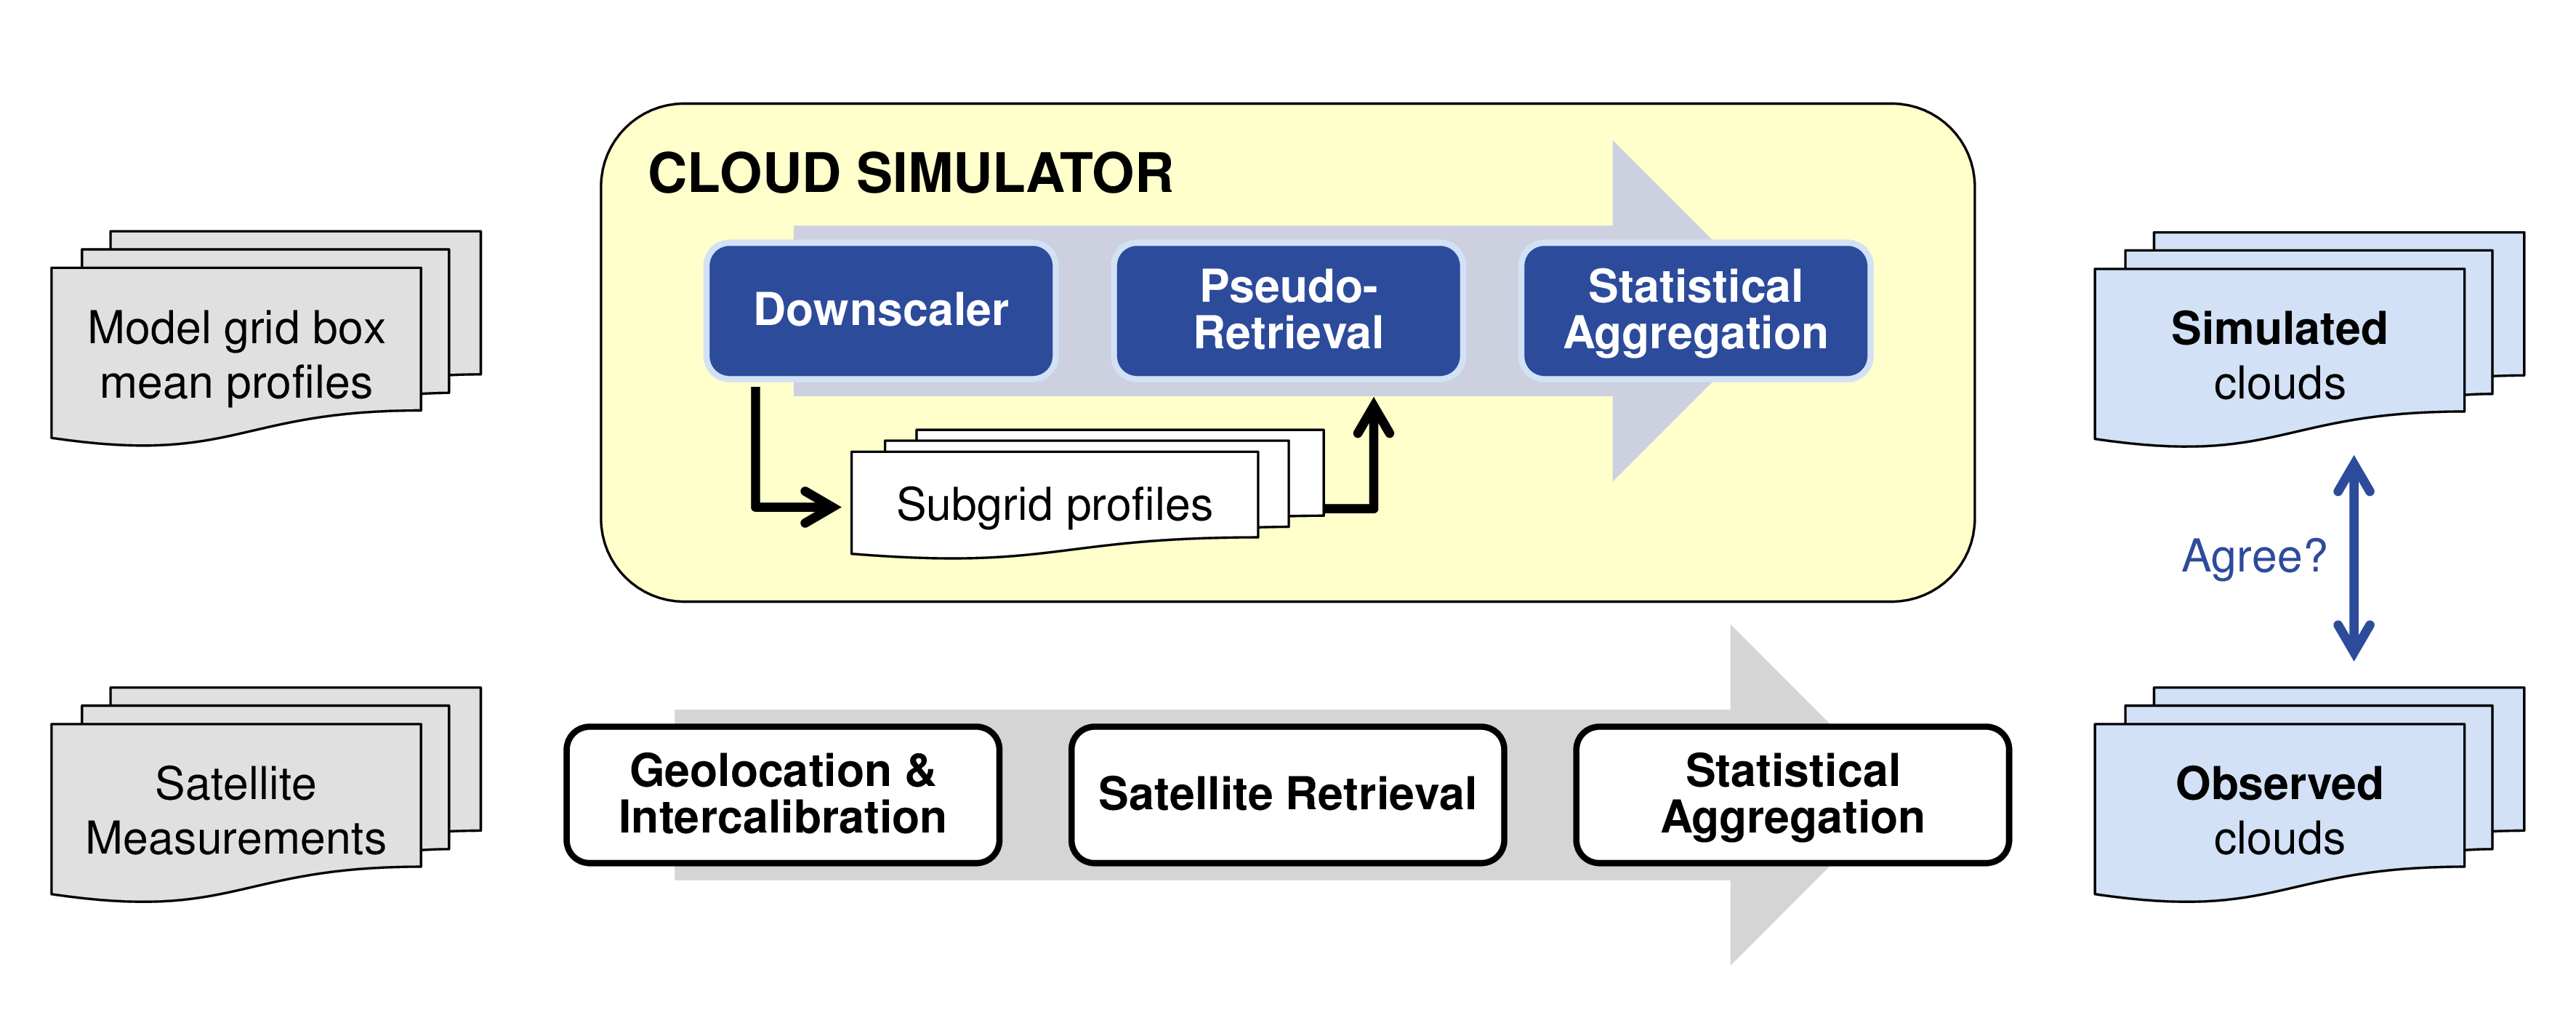
\includegraphics[width=\mapwidth]{./figures/simulator_overview.png}
  \caption[Concept of the cloud simulator.]
{Cloud simulator concept.}\label{fig:sim_over}
\end{figure}


\newpage
\section{Description of datasets}\label{sec:datasets}


\subsection{ERA-Interim reanalysis}\label{sec:era}

The ERA-Interim global atmospheric reanalysis \cite{Dee2011} provided by ECMWF 
(European Centre for Medium-Range Weather Forecasts) 
is the follow-up of ERA-40 reanalysis \cite{Uppala2005}, which was completed in 2002.
It covers the period from 1979 onwards and is continuously extended in near-real time.
One of the main objectives was to solve various difficulties regarding data assimiliation
(e.g. use of satellite data), which were found during the production of ERA-40. 
Evaluations of the new dataset have demonstrated that the hydrological cycle, the stratospheric circulation, and
the consistency in time of the reanalysis fields have been improved.
Data assimilation methodology, forecast model, and input observations
are essential components for the generation of high quality reanalysis data,
and consequently, will lead to more confident results in climate change applications. 

The reanalysis is produced by the Integrated Forecast System (IFS), which includes
the forecast model consisting of three fully coupled components for the atmosphere, land surface, and ocean waves.
ERA-Interim clouds are represented by a fully prognostic cloud scheme where cloud-related processes
are treated in a unified way, i.e. they are physically realistic and consistent with the rest of the model.
The scheme for stratiform and convective clouds has been developed by Tiedtke \cite{Tiedtke1993}, 
implemented in the global forecast model operationally in 1995 and since then, continuously improved.
An important and indispensable limitation of large-scale models is the fact that only bulk
properties of clouds can be taken into account. Hence, clouds are defined by
the horizontal coverage of the grid box by cloud, and the mass mixing ratio of total cloud condensate,
along with the constraint that cloud air is saturated with regard to water and ice, respectively.
The thermodynamic phase is determined on the basis of the temperature.
In other words, cloud cover and cloud water/ice content are derived from prognostic equations,
which follow the mass balance equation for cloud water/ice content and cloud air.
As time evolves in the simulation the cloud variables are changing due to source and
sink terms that are related to cloud formation (e.g., condensation/sublimation, cumulus convection)
and destruction (e.g., evaporation, precipitation) processes, respectively.

% % % A new prognostic bulk microphysics scheme for the ECMWF forecast model
% % % R. M. Forbes (1), A. M. Tompkins (2), and A. Untch (1)
% % % (1) ECMWF, shinfield Park, Reading U.K, (2) ICTP, Earth System Physics, Trieste, Italy (tompkins@ictp.it)
% A major upgrade to the parametrization of stratiform cloud and precipitation was implemented in the Integrated
% Forecast System (IFS) cycle 36r4, operational at ECMWF from 9 November 2010. Three additional prognostic
% variables  have  been  introduced  to  enable  a  more  physically  based  representation  of  mixed-phase  (liquid/ice)
% cloud and precipitating rain and snow. A fully implicit method is employed to solve the network of microphysics
% pathways stably for long timesteps. It is the most significant change to the structure of the cloud parametrization
% since the Tiedtke scheme was introduced operationally in 1995. Many aspects of the model are systematically
% improved including the skill of precipitation forecasts, the spatial distribution of ice and snow in the troposphere,
% the physical processes in mixed-phase cloud and the impact of cloud and precipitation on radiation.

As already metioned above the original Tiedtke scheme has been continuously further developed
aiming at a more physically realistic representation of cloud and precipitation microphysics
that cannot be achieved by using just two prognostic cloud variables.
A revised Tiedtke cloud parameterization of stratiform cloud and precipitation became available by 2010
increasing the number of prognostic variables from two (cloud fraction, cloud condensate) to five
(cloud fraction, cloud liquid water, cloud ice, rain, and snow).
The updated approach treats now water and ice clouds independent leading to more realistic
modelling of supercooled liquid water clouds as well as snow and rain precipitation processes.

% % % taken from Dee et al. 2011 % % %
% Improvements of the model physics have caused a positive impact on the 
% representation of clouds in the ERA-Interim dataset \cite{Dee2011}. By comparing the ERA-Interim and ERA-40 
% reanalysis with ISCCP observations several improvements regarding cloud cover have been identified. 
% For instance, the marine stratocumulus cloud cover has been increased by 15 -- 25~\%
% because a new moist boundary-layer scheme was implemented \cite{Koehler2011}.
% The tropical ocean total cloud cover has been decreased by 5 -- 15~\% 
% due to an overall improved hydrological cycle and the incorporation of ice supersaturation 
% delaying the formation of ice clouds \cite{Tompkins2007}.
% The cloud cover over land in the tropics has been increased by 20 -- 30~\% caused by an
% increase in high cloud resulting from improved deep convective triggering \cite{Bechtold2004} along
% with low cloud produced by a new boundary-layer scheme.
% The midlatitude ocean (low- and medium-height) cloud cover has been increased by about 5~\% due to
% improved numerics of the cloud scheme.

Models and observations are incomplete having uncertainties. Data assimiliation is the process,
which incorporates observations into the model regime generating the optimum atmospheric 
state at a particular time, which is better than that from model or observation on their own.
As a consequence, random errors can be minimized. However, there are also many systematic 
differences between models and observations, which require a careful treatment \cite{Forbes2015}.

\cite{IPCC2013}
In the last two decades significant progress have been made in improving the parameterization 
of clouds in large-scale models. But still assumptions and simplifications are necessary 
limiting the
% In any large-scale model basic assumptions and simplifications are necessary for representing clouds.
% Clouds and also aerosol are still the largest uncertainties in GCMs and thus,
% it is important to further understand the processes and improve their representation in models.
% altough in den last 10 years major progress has been made
% models needs to be evaluated by other models and observations
% retrievals needs to be verified by models
% neither model nor retrievals are perfect due to the complexity of the real world.
% assumptions and limitations are required in both
% make bridge to CC4CL here


\subsection{Cloud\_cci dataset}\label{sec:cloudcci}

The ESA Cloud\_cci project presents new long-term coherent AVHRR and MODIS cloud property datasets 
(1982 – 2014) along with associated uncertainties obtained by optimal estimation theory. 
The algorithm fits a physically consistent cloud/atmosphere/surface model to satellite observations 
simultaneously from the visible to the mid-infrared, thereby ensuring spectral consistency for 
all retrieved and derived parameters. This retrieval scheme, referred to as Community Optimal 
Estimation Cloud Retrieval for Climate (CC4CL), provides cloud fraction, cloud top level estimates, 
cloud thermodynamic phase, cloud optical thickness, cloud effective radius and post processed products, 
such as cloud liquid and ice water path.


\newpage
\section{Cloud simulator description}\label{cld_sim}

%\section{Description of the cloud simulator}\label{simpsimu}

This section describes the main steps of retrieving monthly mean 
Cloud\_cci-like (i.e. pseudo-satellite) observations derived from 
global atmospheric reanalysis produced by ECMWF.
The clouds simulator reads the 6-hourly (00, 06, 12, 18 UTC) 
ERA-Interim files per month containing gridbox mean vertical profiles of
\begin{itemize}
    \setlength\itemsep{0.2em}
    \item pressure level $P_{lev}$ [Pa],
    \item liquid water content $LWC$ [kg/kg]$\footnote{mass of condensate per mass of moist air}$,
    \item ice water content $IWC$ [kg/kg],
    \item cloud cover $CC$ (0-1),
    \item geopotential height $h_{geo}$ [m$^{2}/s^{2}$], and
    \item temperature $T$ [K].
\end{itemize}
A detailed description of the ERA-Interim data is given in section~\ref{sec:era}.
The following steps address the things needed to simulate the observational process.
In other words, what would a satellite see if the atmosphere had the clouds
of a climate model?


%\subsection{Calculation of cloud effective radius, optical thickness and water path}
\subsection{Pre-processing}

In the first step the gridbox mean liquid and ice water contents at each model level
are weighted by the cloud cover profile providing the so-called 
``in-cloud'' liquid and ice water contents. 
Thus, only the cloudy part of the grid cell is taken into account, 
which is comparable to what a satellite would detect.
Based on these cloud-cover-weighted profiles the liquid ($LWP$) and ice ($IWP$) water paths
per model layer can be derived, which present the total amount of liquid and ice
water between two consecutive pressure levels in the atmosphere, respectively.
The total amount of $LWP$ and $IWP$ is referred to as cloud water path ($CWP$).

The cloud optical thickness ($\tau$) per layer is obtained by the method of \citet{Han1994}
\begin{equation}\label{eq:han}
    \tau = \frac{3}{4} \frac{CWP \cdot  Q_{ext}}{r_{e} \cdot \rho}
\end{equation}
where $CWP$ represents either $LWP$ or $IWP$ depending on the thermodynamic phase.
$Q_{ext}$ denotes the extinction coefficient, which is assumed to be 2 for water and 2.1 for ice.
The density $\rho$ is set to 1 $g/m^{3}$ for water and 0.9167 $g/m^{3}$ for ice.
For the computation of effective radii ($r_{e}$) per layer the 
ERA-Interim parameterizations are implemented in the cloud simulator.

The cloud droplet effective radius ($r_{e}^{liq}$) follows the method of \citet{Martin1994} and 
is defined as function of liquid water content and cloud droplet number 
concentration, which in turn depends on the wind speed.
For practical reasons the simulator uses constant values for the number of 
cloud condensation nuclei over land (300) and sea (100).
Hence, a land-sea mask (Fig.~\ref{fig:lsm}) is required, 
which is obtained from ERA-Interim Sea Surface Temperature (Fig.~\ref{fig:sst}) 
data aggregated on a 0.5$^{\circ}$ latitude-longitude grid.
The ice crystal effective radius ($r_{e}^{ice}$) is parameterized as a function of 
temperature and ice water content based on \citet{Sun1999}, which has been
revised by \citet{Sun2001}.

In CC4CL the simultaneously retrieved $\tau^{liq}$ ($\tau^{ice}$) and 
$r_{e}^{liq}$ ($r_{e}^{ice}$) are combined utilizing the relationship given in 
Eq.~\ref{eq:han} for deriving $LWP$ ($IWP$) as post-processed product.
Thus, the cloud simulator adopts this retrieval characteristic of CC4CL by
using this equation for computing the 
cloud optical thickness per model layer since ERA-Interim provides solely 
the information on the cloud water content and cloud amount.

%\captionsetup[subfloat]{position=top}
\begin{figure}[!h]
  \begin{minipage}[t]{0.5\textwidth}
    \subfloat[ERA-Interim land-sea mask (LSM).]
    {\includegraphics[scale=0.26]{./figures/{lsm_era_interim_0.5_0.5}.png}\label{fig:lsm}}
  \end{minipage}
  \begin{minipage}[t]{0.5\textwidth}
    \subfloat[ERA-Interim sea surface temperature (SST).]
    {\includegraphics[scale=0.26]{./figures/{sst_era_interim_0.5_0.5}.png}\label{fig:sst}}
  \end{minipage}
  \caption[ERA-Interim land-sea mask and sea surface temperature (31/08/2015).]
{ERA-Interim auxiliary data provided on a 0.5$^{\circ}$ latitude-longitude grid.}\label{fig:lsm_sst}
\end{figure}


\subsection{Downscaler}
In the next step the simulator has to adress the mismatch in scale between 
that of a ERA-Interim model grid box ($\sim$ 500 km) and 
that of a satellite footprint ($\sim$ 5 km, e.g. AVHRR).
This is achieved by scaling the grid box mean profiles (e.g., 
Fig.~\ref{fig:profiles}) for each grid cell down to subcolumns$\footnote{
Currently each grid cell is broken into 20 subcolumns. This will be changed 
so that the number of subcolumns will be a function of latitude.}$, which
can be thought of as respresenting the spatial resolution of the instrument.
Figure~\ref{fig:scops} shows examples of vertical profiles of individual subcolumns 
for two different grid cells based on the grid box mean profiles displayed in 
Figure~\ref{fig:profiles}.
The upper left figure illustrates the subgrid cloud fraction profiles 
%The downscaler applies a pseudo-random sampling process 
%to generate an ensemble of subgrid profiles, which the distribution within the model grid box.

The cloud simulator assumes maximum random overlap of clouds, which means 
that clouds in neighboring layers are maximally overlapped, 
while groups of clouds separated by one or more clear layers are randomly overlapped.

%This method uses a pseudo-random sampling process to generate an ensemble of subgrid cloud
%profiles representing the distribution within the model grid box. It takes the input vertical
%profiles of cloud fraction to generate a specified number of horizontally homogeneous cloud
%profiles. The SCOPS algorithm splits each grid column into a number of subcolumns NCOL in which
%each layer is either completely filled or completely free of cloud. The cloud cover in each
%vertical layer and subcolumn is therefore either 0 or 1. The SCOPS version used here assumes
%maximum random overlap for cloud

The used approach for deriving subgrid profiles is very similar to
SCOPS (Subgrid Cloud Overlap Profile Sampler, \citet{Webb2001}),
which is implemented, for instance, in COSP (CFMIP Observation Simulator
Package, \cite{Bodas2011}).
COSP is an integrated satellite simulator, which has been developed by 
the Cloud Feedback Model Intercomparison Project (CFMIP) community.
It is capable to simulate observations of multiple active and passive
satellite instruments (e.g., CloudSat, Calipso, ISCCP, MISR, MODIS, RTTOV) 
and therefore, allows the quantitative evaluation of clouds, humidity,
and precipitation processes in diverse numerical models.



% grid box mean profiles 
\begin{figure}[!h]
  \centering
  \begin{minipage}{0.3\textwidth}
    \subfloat[Cloud fraction.]
    {\includegraphics[scale=0.17]{./figures/\snapscops_CFC9_profile.png}}
  \end{minipage}\hfill
  \begin{minipage}{0.3\textwidth}
    \subfloat[Cloud optical thickness.]
    {\includegraphics[scale=0.17]{./figures/\snapscops_COT9_profile.png}}
  \end{minipage}\hfill
  \begin{minipage}{0.3\textwidth}
    \subfloat[Cloud water path.]
    {\includegraphics[scale=0.17]{./figures/\snapscops_CWP9_profile.png}}
  \end{minipage}
  \caption[Grid box mean profiles.]{Example of cloud fraction (a),
cloud optical thickness (b) and cloud water path (c) 
grid box mean profiles. The grid cell is located in the daytime 
(solar zenith angle equal 17.7) at N$31^{\circ}30^{\prime}$ and 
E$164^{\circ}0^{\prime}$ at UTC 00 on 1$^{st}$ of \MonthYear.}
  \label{fig:profiles}
\end{figure}


% subcolumn cloud distribution 
\begin{figure}[!h]
  \centering

  \begin{minipage}{0.3\textwidth}
    \subfloat[Cloud fraction.]
    {\includegraphics[scale=0.17]{./figures/\snapscops_CFC9.png}}
  \end{minipage}\hfill
  \begin{minipage}{0.3\textwidth}
    \subfloat[Cloud optical thickness.]
    {\includegraphics[scale=0.17]{./figures/\snapscops_COT9.png}}
  \end{minipage}\hfill
  \begin{minipage}{0.3\textwidth}
    \subfloat[Cloud water path.]
    {\includegraphics[scale=0.17]{./figures/\snapscops_CWP9.png}}
  \end{minipage}\hfill

  \begin{minipage}{0.3\textwidth}
    \subfloat[Cloud effective radius.]
    {\includegraphics[scale=0.17]{./figures/\snapscops_CER9.png}}
  \end{minipage}\hfill
  \begin{minipage}{0.3\textwidth}
    \subfloat[Cloud phase.]
    {\includegraphics[scale=0.17]{./figures/\snapscops_CPH9.png}}
  \end{minipage}

  \caption[Down-scaled cloud parameter profiles.]{Top-down: 
Subcolumn distribution of cloud fraction, phase, effective radius, 
optical thickness and water path derived from grid box mean profiles
shown in Figure~\ref{fig:profiles} for
two different grid cells at UTC 00 on 1$^{st}$ of \MonthYear.}
  \label{fig:scops}
\end{figure}




%2. search for upper-most cloud and collect cloud parameters
\subsection{Pseudo-retrieval}
operate on subcolumns
%In the previous section the pre-processing of pseudo-satellite 
%$\tau$, $r_{e}$, and $CWP$ vertical profiles has been explained,
%which complement along with the original ERA-Interim 3D fields the required
%input data for the pseudo retrieval.
%This is the essential part of the cloud simulator responsible for producing 
%output comparable to Cloud\_cci data in three main steps.
%Scale COT greater than 100.
%Only solar COT, CWP, CER due to CC4CL.


% cloud top parameters 
\begin{figure}[!h]
  \begin{minipage}{\textwidth}
    \subfloat[Grid cell at N$29^{\circ}30^{\prime}$ and E$162^{\circ}30^{\prime}$.]
    {\includegraphics[width=\textwidth]{./figures/\snapscops_retrieved1.png}}
  \end{minipage}\vspace*{0.5cm}
  \begin{minipage}{\textwidth}
    \subfloat[Grid cell at N$31^{\circ}30^{\prime}$ and E$164^{\circ}0^{\prime}$.]
    {\includegraphics[width=\textwidth]{./figures/\snapscops_retrieved9.png}}
  \end{minipage}
  \caption[Retrieved subcolumn cloud top parameters.]
{Retrieved subcolumn cloud fraction (CFC), cloud top pressure (CTP),
cloud top temperature (CTT), cloud top height (CTH),
cloud phase (CPH), cloud effective radius (CER),
cloud optical thickness (COT), and cloud water path (CWP) 
for two different grid boxes at UTC 00 on 1$^{st}$ of \MonthYear.}
\label{fig:retrieved}
\end{figure}



%3. collect statistics, i.e. means over subcolumns and 1D, 2D histograms
\subsection{Compute summary statistics}


%% CER, CWP, COT only daytime
%\begin{figure}[!h]
%  \begin{minipage}[c]{0.5\textwidth}
%    \includegraphics[scale=0.27]{./figures/{\szamidnight}.png}
%    \includegraphics[scale=0.27]{./figures/{\szamidday}.png}
%  \end{minipage}\hfill
%  \begin{minipage}[c]{0.5\textwidth}
%    \includegraphics[scale=0.27]{./figures/{\szamorning}.png}
%    \includegraphics[scale=0.27]{./figures/{\szaevening}.png}
%  \end{minipage}
%  \caption[Solar zenith angle for 00, 06, 12, 18 UTC.]
%  {Solar zenith angle maps for 00, 06, 12, and 18 UTC on 1$^{st}$ of \MonthYear.} 
%  \label{fig:sza}
%\end{figure}
%
%





%\FloatBarrier
%\section{Simulator results}\label{sec:sim_results}
%\subsection{Pseudo-satellite products for \MonthYear}
%

\begin{figure}[!ht]
  \centering
  \includegraphics[width=\hiswidth]{{\hisout_cer}.png}
  \includegraphics[width=\mapwidth]{{\mapout_cer}.png}
  \caption[Simulated monthly mean cloud effective radius.]
  {Simulated monthly mean cloud effective radius for \MonthYear.} 
  \label{fig:cer}
\end{figure}


\newpage
\begin{figure}[!ht]
  \centering
  \includegraphics[width=\mapwidth]{{\mapout_cer_liq}.png}
  \includegraphics[width=\mapwidth]{{\mapout_cer_ice}.png}
  \caption[Simulated monthly mean liquid and ice cloud effective radius.]
  {Simulated monthly mean liquid and ice cloud effective radius for \MonthYear.} 
  \label{fig:cer_liq_ice}
\end{figure}



\newpage
\begin{figure}[!ht]
  \centering
  \includegraphics[width=\hiswidth]{{\hisout_cot}.png}
  \includegraphics[width=\mapwidth]{{\mapout_cot}.png}
  \caption[Simulated monthly mean cloud optical thickness.]
  {Simulated monthly mean cloud optical thickness for \MonthYear.} 
  \label{fig:cot}
\end{figure}


\newpage
\begin{figure}[!ht]
  \centering
  \includegraphics[width=\mapwidth]{{\mapout_cot_liq}.png}
  \includegraphics[width=\mapwidth]{{\mapout_cot_ice}.png}
  \caption[Simulated monthly mean liquid cloud optical thickness.]
  {Simulated monthly mean liquid cloud optical thickness for \MonthYear.} 
  \label{fig:cot_liq_ice}
\end{figure}



\newpage
\begin{figure}[!ht]
  \centering
  \includegraphics[width=\hiswidth]{{\hisout_cwp}.png}
  \includegraphics[width=\mapwidth]{{\mapout_cwp}.png}
  \caption[Simulated monthly mean cloud water path.]
  {Simulated monthly mean cloud water path for \MonthYear.} 
  \label{fig:cwp}
\end{figure}


\newpage
\begin{figure}[!ht]
  \centering
  \includegraphics[width=\mapwidth]{{\mapout_lwp}.png}
  \includegraphics[width=\mapwidth]{{\mapout_iwp}.png}
  \caption[Simulated monthly mean liquid and ice cloud water path.]
  {Simulated monthly mean liquid and ice cloud water path for \MonthYear.} 
  \label{fig:cwp_liq_ice}
\end{figure}



\newpage
\begin{figure}[!ht]
  \centering
  \includegraphics[width=\hiswidth]{{\hisout_ctp}.png}
  \includegraphics[width=\mapwidth]{{\mapout_ctp}.png}
  \caption[Simulated monthly mean cloud top pressure.]
  {Simulated monthly mean cloud top pressure for \MonthYear.} 
  \label{fig:ctp}
\end{figure}


\newpage
\begin{figure}[!ht]
  \centering
  \includegraphics[width=\hiswidth]{{\hisout_ctt}.png}
  \includegraphics[width=\mapwidth]{{\mapout_ctt}.png}
  \caption[Simulated monthly mean cloud top temperature.]
  {Simulated monthly mean cloud top temperature for \MonthYear.} 
  \label{fig:ctt}
\end{figure}


\newpage
\begin{figure}[!ht]
  \centering
  \includegraphics[width=\mapwidth]{{\mapout_cfc}.png}
  \includegraphics[width=\mapwidth]{{\mapout_cph}.png}
  \caption[Simulated monthly mean cloud fraction and cloud phase.]
  {Simulated monthly mean cloud fraction and cloud phase for \MonthYear.} 
  \label{fig:cfc_cph}
\end{figure}

%
%\FloatBarrier
%%\section{Comparison of simulated and observed cloud parameters}\label{sec:sim_vs_obs}
%\section{Comparison of {\era} vs. {\cci}-{\fv}}\label{sec:sim_vs_obs}
%\subsection{Histograms}
%
%\begin{figure}[!ht]
%  \begin{minipage}[t]{0.4\textwidth}
%    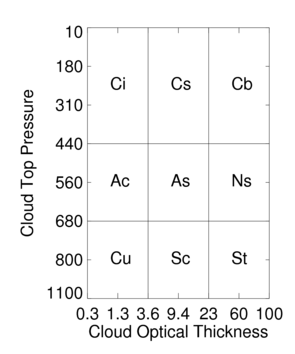
\includegraphics[scale=0.50]{./content/isccp_uebersicht.png} 
%    \caption[ISCCP COT-CTP classification.]{\isccp}\label{fig:isccp}
%  \end{minipage}\hfill
%  \begin{minipage}[c]{0.55\textwidth}
%    \centering
%    \includegraphics[scale=0.20]{\jchdiff}\\
%    \includegraphics[scale=0.20]{\jchdiffliq}\\
%    \includegraphics[scale=0.20]{\jchdiffice} 
%    \caption[Difference Joint cloud proptery histograms.]{\jchdiffcaption}\label{fig:jchdiff}
%  \end{minipage}
%\end{figure}


\begin{figure}[!ht]
  \begin{minipage}[c]{0.4\textwidth}
    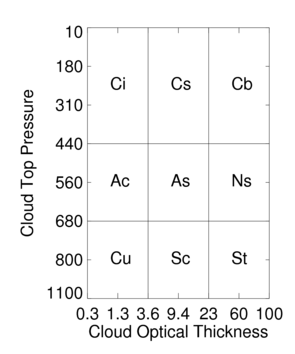
\includegraphics[scale=0.50]{./content/isccp_uebersicht.png} 
  \end{minipage}\hfill
  \begin{minipage}[c]{0.6\textwidth}
    \caption[ISCCP COT-CTP classification.]{\isccp}\label{fig:isccp}
  \end{minipage}
\end{figure}


\begin{figure}[!ht]
  \centering
  \includegraphics[scale=0.19]{\jchdiff} \\
  \includegraphics[scale=0.19]{\jchdiffliq}
  \includegraphics[scale=0.19]{\jchdiffice} 
  \caption[Joint cloud proptery histograms (difference).]{\jchdiffcaption}\label{fig:jchdiff}
\end{figure}

\begin{figure}[!ht]
  \centering
  \includegraphics[scale=0.22]{\jchera} 
  \includegraphics[scale=0.22]{\jchcci} \\
  \includegraphics[scale=0.22]{\jcheraliq}
  \includegraphics[scale=0.22]{\jchcciliq} \\
  \includegraphics[scale=0.22]{\jcheraice}
  \includegraphics[scale=0.22]{\jchcciice} 
  \caption[Joint cloud proptery histograms.]{\jchcaption}
  \label{fig:jch}
\end{figure}



%

\begin{figure}[!ht]
  \centering
  \begin{minipage}{0.5\textwidth}
    \subfloat[Normalized histogram of CTP.]
    {\includegraphics[width=\halffigwidth]{{\hisout_ctp_\vscci}.png}\label{fig:hist1d_ctp}}
  \end{minipage}\hfill
  \begin{minipage}{0.5\textwidth}
    \subfloat[Normalized histogram of CTT.]
    {\includegraphics[width=\halffigwidth]{{\hisout_ctt_\vscci}.png}\label{fig:hist1d_ctt}}
  \end{minipage}\hfill
    \begin{minipage}{0.5\textwidth}
    \subfloat[Normalized histogram of COT.]
    {\includegraphics[width=\halffigwidth]{{\hisout_cot_\vscci}.png}\label{fig:hist1d_cot}}
  \end{minipage}\hfill
  \begin{minipage}{0.5\textwidth}
    \subfloat[Normalized histogram of CWP.]
    {\includegraphics[width=\halffigwidth]{{\hisout_cwp_\vscci}.png}\label{fig:hist1d_cwp}}
  \end{minipage}\hfill
  \begin{minipage}{0.5\textwidth}
    \subfloat[Normalized histogram of CER.]
    {\includegraphics[width=\halffigwidth]{{\hisout_cer_\vscci}.png}\label{fig:hist1d_cer}}
  \end{minipage}\hfill
  \begin{minipage}{0.45\textwidth}
  \caption[One-dimensional normalized histograms.]{Normalized one-dimensional (1D) histograms of
  cloud top pressure (a), cloud top temperature (b), cloud optical thickness (c),
  cloud water path (d), and cloud effective radius (e) 
  derived from {\simversion} and {\cciversion} for {\MonthYear}.
  Each bin is normalized to the total number of retrievals and hence,
  displaying relative frequencies.}\label{fig:hist1d}
  \end{minipage}
\end{figure}



% \begin{figure}[!ht]
%   \centering
%   \includegraphics[width=\hiswidth]{{\hisout_ctp_\vscci}.png}
%   \caption[Cloud top pressure histogram.]
%   {Cloud top pressure histogram {\hiscaption}} 
%   \label{fig:hist1d_ctp}
% \end{figure}
% 
% \begin{figure}[!ht]
%   \centering
%   \includegraphics[width=\hiswidth]{{\hisout_ctt_\vscci}.png}
%   \caption[Cloud top temperature histogram.]
%   {Cloud top temperature histogram {\hiscaption}} 
%   \label{fig:hist1d_ctt}
% \end{figure}
% 
% \begin{figure}[!ht]
%   \centering
%   \includegraphics[width=\hiswidth]{{\hisout_cot_\vscci}.png}
%   \caption[Cloud optical thickness histogram.]
%   {Cloud optical thickness histogram {\hiscaption}} 
%   \label{fig:hist1d_cot}
% \end{figure}
% 
% \begin{figure}[!ht]
%   \centering
%   \includegraphics[width=\hiswidth]{{\hisout_cwp_\vscci}.png}
%   \caption[Cloud water path histogram.]
%   {Cloud water path histogram {\hiscaption}} 
%   \label{fig:hist1d_cwp}
% \end{figure}
% 
% 
% \begin{figure}[!ht]
%   \centering
%   \includegraphics[width=\hiswidth]{{\hisout_cer_\vscci}.png}
%   \caption[Cloud effective radius histogram.]
%   {Cloud effective radius histogram {\hiscaption}} 
%   \label{fig:hist1d_cer}
% \end{figure}


%
%\FloatBarrier
%\subsection{L3C}
%
% ===== LANDSCAPE ======

\begin{landscape}

\begin{figure}[!ht]
  \centering
  \includegraphics[scale=0.35]{{\comparecci_CFC_\era}.png}
  \includegraphics[scale=0.35]{{\comparecci_CFC_\cci}.png}\\
  \includegraphics[scale=0.35]{{\comparecci_CFC_\era_\cci_\histo}.png}
  \includegraphics[scale=0.35]{{\comparecci_CFC_\era_\cci_\zonal}.png}
  \caption[Monthly mean cloud fraction.]
  {Monthly mean cloud fraction (CFC) for \MonthYear. \compcaption} 
  \label{fig:era_cci_cfc}
\end{figure}


\begin{figure}[!ht]
  \centering
  \includegraphics[scale=0.35]{{\comparecci_CPH_\era}.png}
  \includegraphics[scale=0.35]{{\comparecci_CPH_\cci}.png}\\
  \includegraphics[scale=0.35]{{\comparecci_CPH_\era_\cci_\histo}.png}
  \includegraphics[scale=0.35]{{\comparecci_CPH_\era_\cci_\zonal}.png}
  \caption[Monthly mean cloud phase.]
  {Monthly mean cloud phase (CPH) for \MonthYear. \compcaption} 
  \label{fig:era_cci_cph}
\end{figure}


\begin{figure}[!ht]
  \centering
  \includegraphics[scale=0.35]{{\comparecci_CWP_\era}.png}
  \includegraphics[scale=0.35]{{\comparecci_CWP_\cci}.png}\\
  \includegraphics[scale=0.35]{{\comparecci_CWP_\era_\cci_\histo}.png}
  \includegraphics[scale=0.35]{{\comparecci_CWP_\era_\cci_\zonal}.png}
  \caption[Monthly mean cloud water path.]
  {Monthly mean cloud water path (CWP) for \MonthYear. \compcaption} 
  \label{fig:era_cci_cwp}
\end{figure}


\begin{figure}[!ht]
  \centering
  \includegraphics[scale=0.35]{{\comparecci_LWP_\era}.png}
  \includegraphics[scale=0.35]{{\comparecci_LWP_\cci}.png}\\
  \includegraphics[scale=0.35]{{\comparecci_LWP_\era_\cci_\histo}.png}
  \includegraphics[scale=0.35]{{\comparecci_LWP_\era_\cci_\zonal}.png}
  \caption[Monthly mean liquid cloud water path.]
  {Monthly mean liquid cloud water path (LWP) for \MonthYear. \compcaption} 
  \label{fig:era_cci_lwp}
\end{figure}


\begin{figure}[!ht]
  \centering
  \includegraphics[scale=0.35]{{\comparecci_IWP_\era}.png}
  \includegraphics[scale=0.35]{{\comparecci_IWP_\cci}.png}\\
  \includegraphics[scale=0.35]{{\comparecci_IWP_\era_\cci_\histo}.png}
  \includegraphics[scale=0.35]{{\comparecci_IWP_\era_\cci_\zonal}.png}
  \caption[Monthly mean ice cloud water path.]
  {Monthly mean ice cloud water path (IWP) for \MonthYear. \compcaption} 
  \label{fig:era_cci_iwp}
\end{figure}


\begin{figure}[!ht]
  \centering
  \includegraphics[scale=0.35]{{\comparecci_COT_\era}.png}
  \includegraphics[scale=0.35]{{\comparecci_COT_\cci}.png}\\
  \includegraphics[scale=0.35]{{\comparecci_COT_\era_\cci_\histo}.png}
  \includegraphics[scale=0.35]{{\comparecci_COT_\era_\cci_\zonal}.png}
  \caption[Monthly mean cloud optical thickness.]
  {Monthly mean cloud optical thickness (COT) for \MonthYear. \compcaption} 
  \label{fig:era_cci_cot}
\end{figure}


\begin{figure}[!ht]
  \centering
  \includegraphics[scale=0.35]{{\comparecci_COT_LIQ_\era}.png}
  \includegraphics[scale=0.35]{{\comparecci_COT_LIQ_\cci}.png}\\
  \includegraphics[scale=0.35]{{\comparecci_COT_LIQ_\era_\cci_\histo}.png}
  \includegraphics[scale=0.35]{{\comparecci_COT_LIQ_\era_\cci_\zonal}.png}
  \caption[Monthly mean liquid cloud optical thickness.]
  {Monthly mean liquid cloud optical thickness (COT\_LIQ) for \MonthYear. \compcaption} 
  \label{fig:era_cci_cot_liq}
\end{figure}


\begin{figure}[!ht]
  \centering
  \includegraphics[scale=0.35]{{\comparecci_COT_ICE_\era}.png}
  \includegraphics[scale=0.35]{{\comparecci_COT_ICE_\cci}.png}\\
  \includegraphics[scale=0.35]{{\comparecci_COT_ICE_\era_\cci_\histo}.png}
  \includegraphics[scale=0.35]{{\comparecci_COT_ICE_\era_\cci_\zonal}.png}
  \caption[Monthly mean ice cloud optical thickness.]
  {Monthly mean ice cloud optical thickness (COT\_ICE) for \MonthYear. \compcaption} 
  \label{fig:era_cci_cot_ice}
\end{figure}


\begin{figure}[!ht]
  \centering
  \includegraphics[scale=0.35]{{\comparecci_\cerstring_\era}.png}
  \includegraphics[scale=0.35]{{\comparecci_\cerstring_\cci}.png}\\
  \includegraphics[scale=0.35]{{\comparecci_\cerstring_\era_\cci_\histo}.png}
  \includegraphics[scale=0.35]{{\comparecci_\cerstring_\era_\cci_\zonal}.png}
  \caption[Monthly mean cloud effective radius.]
  {Monthly mean cloud effective radius (CER) for \MonthYear. \compcaption} 
  \label{fig:era_cci_cer}
\end{figure}


\begin{figure}[!ht]
  \centering
  \includegraphics[scale=0.35]{{\comparecci_\cerstring_LIQ_\era}.png}
  \includegraphics[scale=0.35]{{\comparecci_\cerstring_LIQ_\cci}.png}\\
  \includegraphics[scale=0.35]{{\comparecci_\cerstring_LIQ_\era_\cci_\histo}.png}
  \includegraphics[scale=0.35]{{\comparecci_\cerstring_LIQ_\era_\cci_\zonal}.png}
  \caption[Monthly mean liquid cloud effective radius.]
  {Monthly mean liquid cloud effective radius (CER\_LIQ) for \MonthYear. \compcaption} 
  \label{fig:era_cci_cer_liq}
\end{figure}


\begin{figure}[!ht]
  \centering
  \includegraphics[scale=0.35]{{\comparecci_\cerstring_ICE_\era}.png}
  \includegraphics[scale=0.35]{{\comparecci_\cerstring_ICE_\cci}.png}\\
  \includegraphics[scale=0.35]{{\comparecci_\cerstring_ICE_\era_\cci_\histo}.png}
  \includegraphics[scale=0.35]{{\comparecci_\cerstring_ICE_\era_\cci_\zonal}.png}
  \caption[Monthly mean ice cloud effective radius.]
  {Monthly mean ice cloud effective radius (CER\_ICE) for \MonthYear. \compcaption} 
  \label{fig:era_cci_cer_ice}
\end{figure}


\begin{figure}[!ht]
  \centering
  \includegraphics[scale=0.35]{{\comparecci_CTP_\era}.png}
  \includegraphics[scale=0.35]{{\comparecci_CTP_\cci}.png}\\
  \includegraphics[scale=0.35]{{\comparecci_CTP_\era_\cci_\histo}.png}
  \includegraphics[scale=0.35]{{\comparecci_CTP_\era_\cci_\zonal}.png}
  \caption[Monthly mean cloud top pressure.]
  {Monthly mean cloud top pressure (CTP) for \MonthYear. \compcaption} 
  \label{fig:era_cci_ctp}
\end{figure}


\begin{figure}[!ht]
  \centering
  \includegraphics[scale=0.35]{{\comparecci_CTT_\era}.png}
  \includegraphics[scale=0.35]{{\comparecci_CTT_\cci}.png}\\
  \includegraphics[scale=0.35]{{\comparecci_CTT_\era_\cci_\histo}.png}
  \includegraphics[scale=0.35]{{\comparecci_CTT_\era_\cci_\zonal}.png}
  \caption[Monthly mean cloud top temperature.]
  {Monthly mean cloud top temperature (CTT) for \MonthYear. \compcaption} 
  \label{fig:era_cci_ctt}
\end{figure}


\begin{figure}[!ht]
  \centering
  \includegraphics[scale=0.35]{{\comparecci_CTH_\era}.png}
  \includegraphics[scale=0.35]{{\comparecci_CTH_\cci}.png}\\
  \includegraphics[scale=0.35]{{\comparecci_CTH_\era_\cci_\histo}.png}
  \includegraphics[scale=0.35]{{\comparecci_CTH_\era_\cci_\zonal}.png}
  \caption[Monthly mean cloud top height.]
  {Monthly mean cloud top height (CTH) for \MonthYear. \compcaption} 
  \label{fig:era_cci_cth}
\end{figure}

\end{landscape}

% ===== LANDSCAPE ======

%
%\FloatBarrier
%\subsection{Zonal mean inter-comparison for \MonthYear}
%
\begin{figure}[!ht]
  \centering
  \begin{minipage}{0.5\textwidth}
    \subfloat[CFC.]
    {\includegraphics[width=\halffigwidth]{{\zonout_cfc}.png}\label{fig:zonal_cfc}}
  \end{minipage}\hfill
  \begin{minipage}{0.5\textwidth}
    \subfloat[CPH.]
    {\includegraphics[width=\halffigwidth]{{\zonout_cph}.png}\label{fig:zonal_cph}}
  \end{minipage}\hfill
    \begin{minipage}{0.5\textwidth}
    \subfloat[CTP.]
    {\includegraphics[width=\halffigwidth]{{\zonout_ctp}.png}\label{fig:zonal_ctp}}
  \end{minipage}\hfill
  \begin{minipage}{0.5\textwidth}
    \subfloat[CTT.]
    {\includegraphics[width=\halffigwidth]{{\zonout_ctt}.png}\label{fig:zonal_ctt}}
  \end{minipage}\hfill
  \begin{minipage}{0.5\textwidth}
    \subfloat[CTH.]
    {\includegraphics[width=\halffigwidth]{{\zonout_cth}.png}\label{fig:zonal_cth}}
  \end{minipage}\hfill
  \begin{minipage}{0.45\textwidth}
  \caption[Monthly zonal mean inter-comparison of cloud fraction, cloud phase, and cloud top estimates.]{ 
  {\szoncaption} cloud fraction (a), cloud phase (b), cloud top pressure (c),
  cloud top temperature (d), and cloud top height (e) 
  for {\MonthYear} {\ezoncaption} }\label{fig:zonal_means_tops}
  \end{minipage}
\end{figure}



\begin{figure}[!ht]
  \centering
  \begin{minipage}{0.5\textwidth}
    \subfloat[CER.]
    {\includegraphics[width=\halffigwidth]{{\zonout_cer}.png}\label{fig:zonal_cer}}
  \end{minipage}\hfill
  \begin{minipage}{0.5\textwidth}
    \subfloat[liquid CER.]
    {\includegraphics[width=\halffigwidth]{{\zonout_cer_liq}.png}\label{fig:zonal_cer_liq}}
  \end{minipage}\hfill
    \begin{minipage}{0.5\textwidth}
    \subfloat[ice CER.]
    {\includegraphics[width=\halffigwidth]{{\zonout_cer_ice}.png}\label{fig:zonal_cer_ice}}
  \end{minipage}\hfill
  \begin{minipage}{0.45\textwidth}
  \caption[Monthly zonal mean inter-comparison of cloud effective radius.]{ {\szoncaption}
  cloud effective radius (a), liquid cloud effective radius (b), 
  and ice cloud effective radius (c) 
  for {\MonthYear} {\ezoncaption} }\label{fig:zonal_means_cer}
  \end{minipage}
\end{figure}




\begin{figure}[!ht]
  \centering
  \begin{minipage}{0.5\textwidth}
    \subfloat[COT.]
    {\includegraphics[width=\halffigwidth]{{\zonout_cot}.png}\label{fig:zonal_cot}}
  \end{minipage}\hfill
  \begin{minipage}{0.5\textwidth}
    \subfloat[liquid COT.]
    {\includegraphics[width=\halffigwidth]{{\zonout_cot_liq}.png}\label{fig:zonal_cot_liq}}
  \end{minipage}\hfill
    \begin{minipage}{0.5\textwidth}
    \subfloat[ice COT.]
    {\includegraphics[width=\halffigwidth]{{\zonout_cot_ice}.png}\label{fig:zonal_cot_ice}}
  \end{minipage}\hfill
  \begin{minipage}{0.45\textwidth}
  \caption[Monthly zonal mean inter-comparison of cloud optical thickness.]{ {\szoncaption}
  cloud optical thickness (a), liquid cloud optical thickness (b), 
  and ice cloud optical thickness (c) 
  for {\MonthYear} {\ezoncaption} }\label{fig:zonal_means_cot}
  \end{minipage}
\end{figure}




\begin{figure}[!ht]
  \centering
  \begin{minipage}{0.5\textwidth}
    \subfloat[CWP.]
    {\includegraphics[width=\halffigwidth]{{\zonout_cwp}.png}\label{fig:zonal_cwp}}
  \end{minipage}\hfill
  \begin{minipage}{0.5\textwidth}
    \subfloat[LWP.]
    {\includegraphics[width=\halffigwidth]{{\zonout_lwp}.png}\label{fig:zonal_lwp}}
  \end{minipage}\hfill
    \begin{minipage}{0.5\textwidth}
    \subfloat[IWP.]
    {\includegraphics[width=\halffigwidth]{{\zonout_iwp}.png}\label{fig:zonal_iwp}}
  \end{minipage}\hfill
  \begin{minipage}{0.45\textwidth}
  \caption[Monthly zonal mean inter-comparison of cloud water path.]{ {\szoncaption}
  cloud water path (a), liquid cloud water path (b), and ice cloud water path (c) 
  for {\MonthYear} {\ezoncaption} }\label{fig:zonal_means_cwp}
  \end{minipage}
\end{figure}




\newpage
\addcontentsline{toc}{section}{References}
\bibliography{shorttitles,database}
%\bibliography{longtitles,database}

\end{document}
